

\tikzset{every picture/.style={line width=0.75pt}} %set default line width to 0.75pt        

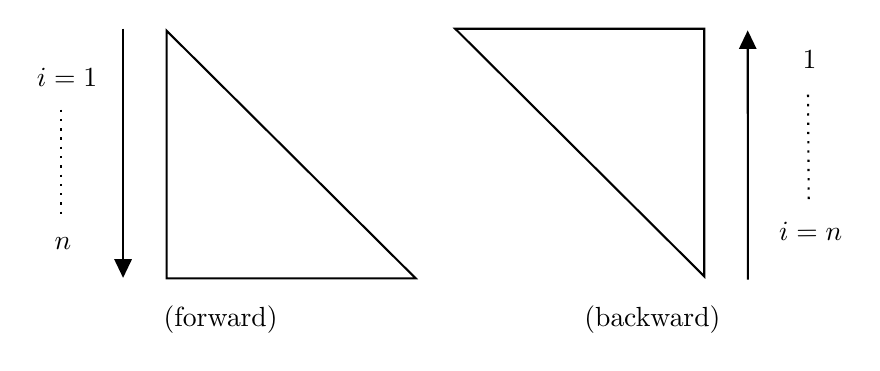
\begin{tikzpicture}[x=0.75pt,y=0.75pt,yscale=-1,xscale=1]
%uncomment if require: \path (0,170); %set diagram left start at 0, and has height of 170

%Shape: Right Triangle [id:dp5671683907330274] 
\draw   (201,11.71) -- (321,131) -- (201,131) -- cycle ;
%Straight Lines [id:da39919664072609184] 
\draw    (180,10.71) -- (180,128.71) ;
\draw [shift={(180,130.71)}, rotate = 270] [fill={rgb, 255:red, 0; green, 0; blue, 0 }  ][line width=0.75]  [draw opacity=0] (8.93,-4.29) -- (0,0) -- (8.93,4.29) -- cycle    ;

%Straight Lines [id:da8365689488016284] 
\draw  [dash pattern={on 0.84pt off 2.51pt}]  (150,49.71) -- (150,100.71) ;



%Shape: Right Triangle [id:dp24623033400831917] 
\draw   (460,130) -- (340,10.71) -- (460,10.71) -- cycle ;
%Straight Lines [id:da8106199446608251] 
\draw    (481.05,131.54) -- (480.95,13.54) ;
\draw [shift={(480.95,11.54)}, rotate = 449.95] [fill={rgb, 255:red, 0; green, 0; blue, 0 }  ][line width=0.75]  [draw opacity=0] (8.93,-4.29) -- (0,0) -- (8.93,4.29) -- cycle    ;

%Straight Lines [id:da46079427117101157] 
\draw  [dash pattern={on 0.84pt off 2.51pt}]  (510.34,92.76) -- (510,41.71) ;





% Text Node
\draw (153,34) node   {$i=1$};
% Text Node
\draw (151,114) node   {$n$};
% Text Node
\draw (511.22,108.46) node [rotate=-359.54]  {$i=n$};
% Text Node
\draw (510.82,25.47) node [rotate=-0.41]  {$1$};
% Text Node
\draw (227,151) node  [align=left] {(forward)};
% Text Node
\draw (435,151) node  [align=left] {(backward)};


\end{tikzpicture}
